\chapter{This is chapter three}


\section{This is section one}

This is some text. This is some text. This is some text. This is some text. This is some text. This is some text. This is some text. 
This is some text. This is some text. This is some text. This is some text. This is some text. This is some text. This is some text. 
The figure~\ref{fig:lena3} is the picture of Lena.
This is some text. This is some text. This is some text. This is some text. This is some text. This is some text. This is some text. 
This is some text. This is some text. This is some text. This is some text. This is some text. This is some text. This is some text. 
This is a reference to a paper~\cite{Garcia_2008_CVGPU}.

\begin{figure}[htbp]
    \centering
    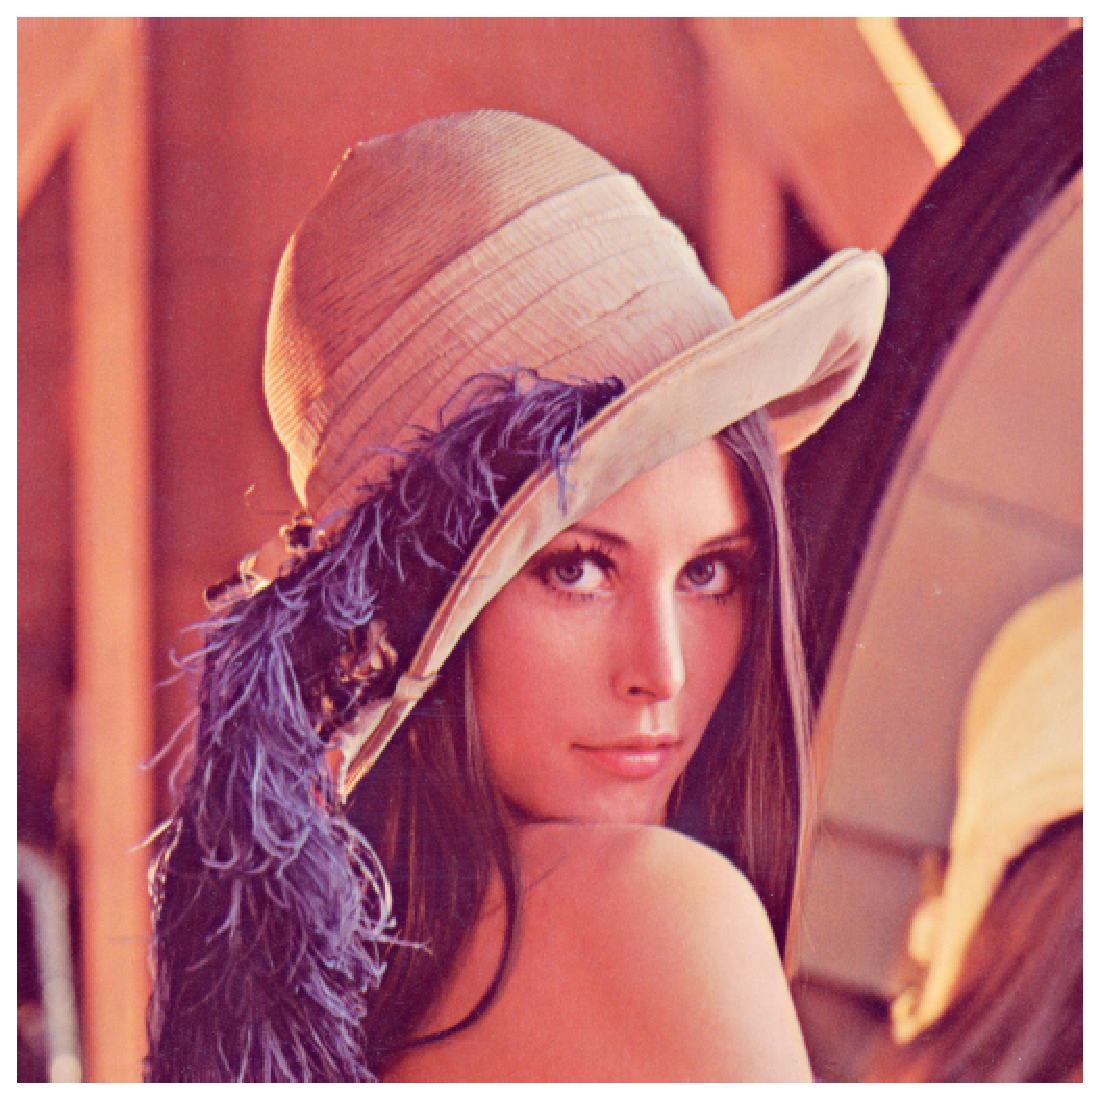
\includegraphics[width=0.4\linewidth]{lena}
    \caption{This is the caption of the figure Lena}
    \label{fig:lena3}
\end{figure}


\section{This is section two}

This is some text. This is some text. This is some text. This is some text. This is some text. This is some text. This is some text. 
This is some text. This is some text. This is some text. This is some text. This is some text. This is some text. This is some text. 
Equation~\ref{eq:normal3} is the formula of a multivariate normal distribution.
This is some text. This is some text. This is some text. This is some text. This is some text. This is some text. This is some text. 
This is some text. This is some text. This is some text. This is some text. This is some text. This is some text. This is some text. 

\begin{equation}
    f_X(x) = \frac{1}{ (2\pi)^{k/2}|\Sigma|^{1/2} } \exp\!\Big( {-\tfrac{1}{2}}(x-\mu)'\Sigma^{-1}(x-\mu) \Big)
    \label{eq:normal3}
\end{equation}


\section{This is section three}

This is some text. This is some text. This is some text. This is some text. This is some text. This is some text. This is some text. 
This is some text. This is some text. This is some text. This is some text. This is some text. This is some text. This is some text. 
The figure~\ref{fig:regularization3} shows some typical functions used in regularization.
This is some text. This is some text. This is some text. This is some text. This is some text. This is some text. This is some text. 
This is some text. This is some text. This is some text. This is some text. This is some text. This is some text. This is some text. 

\begin{figure}[htbp]
    \centering
    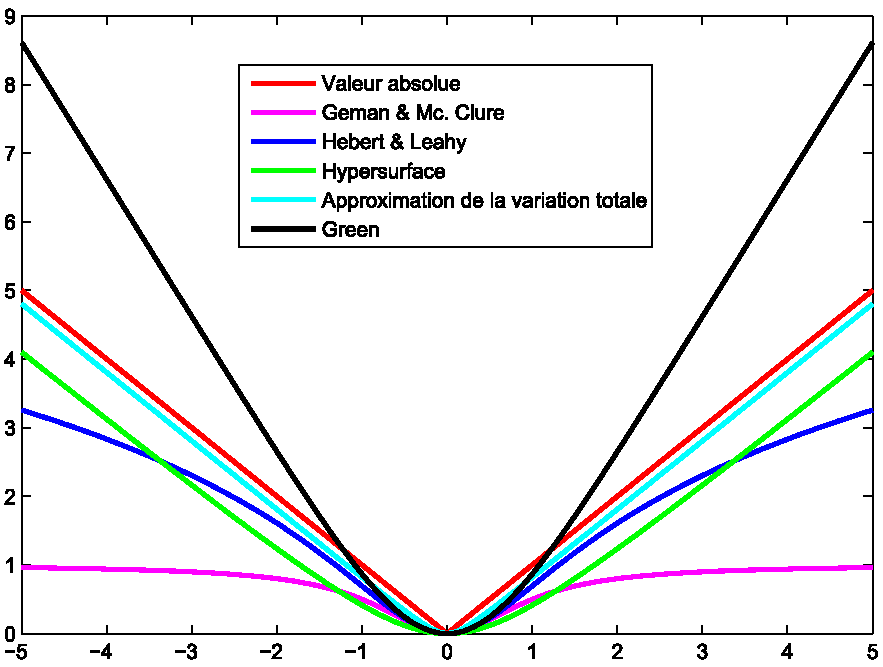
\includegraphics[width=0.7\linewidth]{regularization}
    \caption{Regularization functions}
    \label{fig:regularization3}
\end{figure}